\subsubsection{situacion de pompetitividad entre jovenes}

{\textbf {Resumen:}}
Dos estudiantes están compartiendo y mostrando el uno al otro las piezas que han encontrado en sus museos virtuales, cuando alguno de ellos tiene una pieza que el otro no este le explica en qué parte del museo virtual está y generan una conversación en base a la pieza historica.

{\textbf {Actores:}}
Estudiante-1, Eestudiante-2.

{\textbf {Propósito:}}
Mostrar el uso social de la aplicación dentro del colegio y usar la competitividad como herramienta de aprendizaje.

{\textbf {Referencias cruzadas:}}
R1.1,R1.2, R6.1, R6.2, R6.3, R6.4, R6.6

\paragraph{Caso de Uso Esencial}

\begin{longtable}{|p{5cm}|p{8cm}|}
\hline 
Acción actores & Respuesta del sistema \\ 
\hline 
XXXX & XXXX \\ 
\hline 
\end{longtable}

\paragraph{Diagrama de Caso de Uso}

\begin{figure}[H]
\centerline{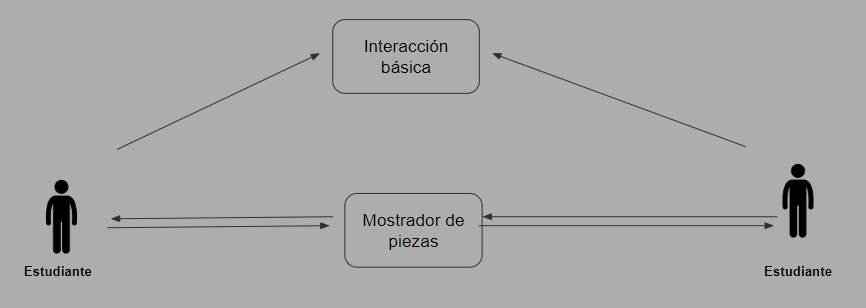
\includegraphics[width=15cm]{imgs/CasoUso_3.PNG}}
\caption{Caso-1}
\label{fig}
\end{figure}

\paragraph{Modelo Conceptual}

%\begin{figure}[H]
%\centerline{\includegraphics[width=15cm]{imgs/CasoUso_1_3.PNG}}
%\caption{Caso-1}
%\label{fig}
%\end{figure}

\paragraph{Diagrama de Secuencia o Colaboración}

\begin{figure}[H]
\centerline{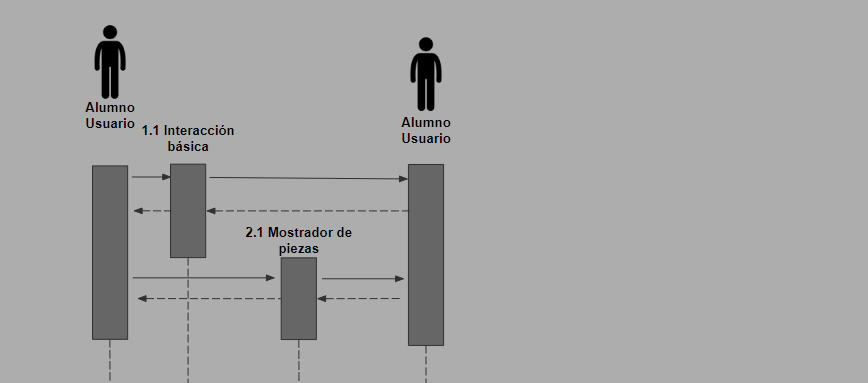
\includegraphics[width=15cm]{imgs/CasoUso_3_2.PNG}}
\caption{Caso-1}
\label{fig}
\end{figure}

\paragraph{Priorización}
{\textbf {Tipo:}}
Relevante.